\documentclass[9pt,twoside,lineno]{pnas-new}
% Use the lineno option to display guide line numbers if required.
\usepackage{subcaption}
\usepackage[figuresleft]{rotating}
\usepackage{fixme}
\usepackage{tikz,bm, amsmath}
\usetikzlibrary{arrows,calc}
\tikzset{
%Define standard arrow tip
>=stealth',
%Define style for different line styles
help lines/.style={dashed, thick},
axis/.style={<->},
important line/.style={thick},
connection/.style={thick, dotted},
}
\graphicspath{{../plots/}}

\templatetype{pnassupportinginfo}
%\readytosubmit %% Uncomment this line before submitting, so that the instruction page is removed.

\title{The Wisdom and Manipulability of Threads}
\author{Robin Engelhardt, Jacob Stærk-Østergaard, Vincent F. Hendricks}
\correspondingauthor{E-mail: robin@hum.ku.dk}

\begin{document}

%% Comment/remove this line before generating final copy for submission
%\instructionspage  

\maketitle

%% Adds the main heading for the SI text. Comment out this line if you do not have any supporting information text.
\SItext

\subsection*{Experimental Setup}
Controlled lab experiments of thread dynamics are rare in the research literature due to the difficulties in keeping a large number of participants in a queue. We designed our experiment along the same lines as the classical information cascade laboratory experiments by Anderson and Holt  that were created to understand student's decision-making behavior in in a sequential decision structure where it can become sensible to ignore private signals due to the aggregation of public knowledge about preceding decisions \cite{anderson1997information}. While such a design is not very feasible in normal laboratory conditions (at least for threads with several hundred participants), it is well suited for online labor markets and crowdsourcing platforms such as Amazon Mechanical Turk (Mturk), an online labor markets and crowdsourcing platform that has become a highly valued tools for social scientists who wish to conduct experimental research on the real time dynamics of large groups. Mturk has repeatedly been shown to meet or exceed the standards set by data collection methods using other means \cite{berinsky2012evaluating, buhrmester2018evaluation}. The platform provides an integrated participant compensation system, has a large participant pool, and has been shown to be reliable, replicable, and significantly more diverse than typical American college samples \cite{mason2009financial, buhrmester2011amazon, crump2013evaluating, rand2012promise, horton2011online}.

Our experimental setup on Mturk is simple. After accepting our ‘HIT’ (Mturk acronym for a ‘human intelligence task’) and providing informed consent, participants are asked to wait in a ‘waiting room’ until the ‘choice room’ (through which all participants have to go sequentially) becomes available. After entering the choice room, participants are asked to take a look at the image and make an estimate (see screenshot in Figure~\ref{fig:S1}).

Depending on the view condition, participants can see $v\in\{0,1,3,9\}$ preceding estimates. We chose to present the ‘oldest’ previous estimate on the top of the list and the last estimate made on the bottom. When dealing with news, or financial data, users typically want to see the most recent activity first (think tweets, online banking transactions, news updates). With conversations it is different because there is a context to consider of whatever message came before and after the one you are looking at (think blogs or facebook comments). We have chosen to use the conversation thread design (oldest on top) because there is no particular news criteria when guessing the weight of an ox or estimating the number of dots on a screen.

Participants have one minute to think about the image and make their estimate. This might sound as a severe time constraint, but exploratory trials had shown that participants in general use less than a minute when performing this task. After submission, participants are thanked for their participation and the experiment ends. Waiting times are compensated with \$0.20 per minute (maximally 5 minutes), participation fee is \$0.10, and a bonus of \$1 is paid if an estimate is within 10\% of the true number.

\subsection*{Mturk Settings and Data Quality}
When working with Mturk it is important to consider the right settings in order to get the best data quality possible \cite{chandler2016conducting}. Fair wage, attrition rates, removal of duplicate participants and informative feedback are some of the most important issues to address.

Average wage for participants in our experiments was $\sim$ \$12 per hour, which is considered good according to Mturk guidelines and certainly above the estimated average of \$6 per hour when excluding un-submitted and rejected work \cite{hara2018data}.

Quitting a study before completing it is prevalent on Mturk, and varies systemically across experimental conditions \cite{zhou2016pitfall}. On average 20 participants accepted our HITs within the first minute; after 10 minutes the average acceptance rate had dropped to 2-3 participants per minute and after an hour to less than one participant per minute. Our scripts were coded in such a way that participants were automatically assigned to a ‘waiting room’ in which they were asked to wait for maximally five minutes before entering the choice room. This meant that a lot of participants waited in vain. Due to such a high attrition rate in the first couple of experiments we changed the script slightly later on: Now the waiting room could contain a maximum of five participants, and when the waiting room was full, participants were told to come back and finish the HIT at a later point in time. This reduced the attrition rate to 6.5\% on average.

All participants automatically received an image-specific qualification when accepting a HIT. This qualification ensured that participants could not accept any other HITs that use the same image. Further data inspection showed that 32 participants somehow managed to accept two HITs with the same image anyway. The reason may be that the time interval between accepting two HITs with the same image was too short for the qualification to register in the Mturk interface. All 32 duplicate participants were removed before data analysis. In addition, we set the qualification that participants should have completed at least 100 HITs and have an accepted HIT rate of 98\% or above. This ensured that we would get only experienced and qualified participants.

Mturk participant attention was expected to be equal to or better than undergraduate participant’s attention \cite{hauser2016attentive}, while various forms of dishonesty (practical joking or telling others about the true value offline or on an Mturk participants web page) was expected to be rare. Our screening of data files before data analyses revealed that a small fraction of participants submitted ridiculously high estimates across images seen, thereby skewing thread averages substantially. These estimates were not treated differently, however, because we had no reason to conclude that they were made with bad intent, and they would be part of the social information given to other participants.

During our experiments, participants had easy access to our email for questions and possible bug reports. Apart from some minor difficulties when typing from a mobile device (less than 1\%) participants had few comments or complaints.

%\subsection*{Code and Software}
%All experiments are coded in the experimental software otree 2.1 \cite{chen2016otree} which is based on python and django. The code itself is designed along the same lines as the classical information cascade experiments by Anderson and Holt \cite{anderson1997information}. The main feature of any cascade game is that decisions are taken sequentially. A player makes an estimate, and the next one receives the information about the estimate of the previous player (or all or some previous players). Thus, the main technical issue is that only one person at a time can make a decision while others wait. As soon as a player finishes and leaves the choice page, the next player enters while all subsequent players still have to wait. Scripts for the analysis of data and for the plotting of all figures in the main text as well as in the Supplementary Information are available on \href{https://github.com/gavstrik/WoT}{github}.

\subsection*{Data Collection}
\label{dc}
We obtained a total of 11748 estimates from 6196 unique participants. Any dot-image was only seen once by a participant, i.e. we had a total of 3157 participants seeing only one image, 1259 participants seeing two images, 1047 participants seeing three images, and 733 participants seeing all four images (either in the unmanipulated or manipulated conditions and with $v\in\{0,1,3,9\}$). A few of the manipulated threads were stopped prematurely (containing less than 100 participants) because early outlier estimates turned the social information available to the succeeding participants into unbelievably high numbers. In those threads, the transition period from compromizing to not at all believing the social information became very short, making the thread dynamics relative uninteresting. Instead of running a highly manipulated thread for a long time, we opted for restarting the thread with new participants. See Table~\ref{table:S1} for a full list of threads and their summary statistics. 

%\subsection*{Outliers}
%Previous work has shown that distributions of independent estimates are approximately log-normal. Consequently, the arithmetic mean is usually much larger than most estimates and often larger than the true value. Testing our data we find distributions to be only approximately log-normal (see QQ-plots in Figure~\ref{fig: qq plots median}). In addition, Table~\ref{table:S1} shows highly variable distributions of estimates. Skewnesses and kurtoses, describing the lack of symmetry and the size of the tail of the distributions, span values from close to zero to above 100. These asymmetries are reflected by the presence of outliers. 
%
%We did not remove any outlier, because the aggregate analysis and linear regression of thread medians is unaffected by the presence of outliers, except for possible larger confidence intervals. We 
%%For all reported aggregate measures, outliers are removed if they have an error rate above 10, so that $|x_r-truth|/truth <10$, where $x_r$ is the estimate by participant $r$. We also use a lower bound of $truth/10$, due some reports of not being able to see the form input on mobile devices or unanticipated timeouts (see SI Appendix, section “Mturk Settings”). With these trimming criteria in place, we count a the following number of outliers: In the dots-experiments, 62 participants have an error rate above 100, and 118 participants have an error rate above 10, while 33 participants have made an estimate below 10\% of the true value. In the ox-experiments, one participant has an error rate above 30 and 9 participants have an error rate above 10, while 94 participants have made an estimate less than 10\% of the true value. This give a total of 151 (1.8 \%) outliers in the dots-experiments and 103 (4.1 \%) outliers in the ox-experiments, giving a grand total of 254 (2.4 \%) outliers out of 10.808 estimates.


\section*{Statistical Methods}
\subsection*{Analysis of thread medians}
The medians were modeled as a linear normal models for the history and manipulated series separately, where the mean in each case was specified as
\begin{align*}
	\mu_{dv} = \alpha_v+\beta_v\log(d), \quad d=55, 148, 403, 1097, \enskip v=0,1,3,9 .
\end{align*}
Hence, the number of views is treated as categorical, since there were clearly an effect of different views, but it was hard to quantify the relationship between different number of views. The ($\log$) number of visible dots was modeled as a quantitative variable, since the distance between $\log(d)$ were deemed suitable scores for this variable. This was also chosen to lower the number of variables in the model, due to the low number of observations (medians) available. 

The models were assessed by quantile-quantile (QQ) and residual plots, as shown in Figure~\ref{fig: qq plots median}. Although some deviation is present, with the available number of observations we do not discard the models based on these plots. The low number of observations in turn implies wide confidence bands as a result, hence conclusions from the models can be viewed as conservative. 

\subsection*{GMM model for social influence}
A Gaussian Mixture Model (GMM) was used model to cope with the heavy tails present in the data. The GMM employs a fixed number of states to fit a weighted sum of gaussian distributions for each observation, hence the \emph{mixture} labeling.

Let $X=\{1,\dots,k\}$ denote the state variable and $Y$ the observation. Then, conditional on $X=j, j=1,\dots,k$, $Y$ follows a normal distribution
\begin{align*}
	Y|(X=j)  \sim \mathcal{N} (\mu_j,\sigma^2_j), j=1,\dots,k,
\end{align*}
hence the unconditional distribution of $Y$ is obtained by integrating (i.e. summing since $X$ is discrete) over $X$
\begin{align*}
	P(Y) = \sum_{j=1}^k P(X=j)P(Y|X=j).
\end{align*}
Including social information as an observed variable in the model, $Y_i$ depends on both $X_i$ and $M_i$, if $v>0$. Furthermore, if $v>1$, then $Y_i$ influences $M_{i+1}$ as the next participant $Y_{i+1}$ will see the estimate of $Y_i$ (assuming the history provide is the previous views).
%Fig. \ref{fig: GMM dependencies} shows a graphical presentation of the model (with preceding views available).
%\begin{figure}[!h]
%\centering
%	\begin{tikzpicture}[->,>=stealth',shorten >=5pt,auto,node distance=3cm, thick,main 	node/.style={circle,fill=gray!25,draw,font=\sffamily\bfseries, minimum size=1.25cm}]
%
%	\node[main node] (x1) {$X_{i}$};
%	%\node[main node] (x2) [right of=x1] {$X_{i+1}$};
%
%	\node[main node] (y1) [below of=x1] {$Y_{i}$};
%	%\node[main node] (y2) [below of=x2] {$Y_{i+1}$};
%
%	\node[main node] (m1) [below of=y1] {$M_{i}$};
%	\node[main node] (m2) [right of=m1] {$M_{i+1}$};
%
%	\path[every node/.style={font=\sffamily\small}]
%    		%(m1) edge [dashed, bend right=30] (m2) 
%    		(m1) edge [dashed] (m2) edge [dashed] (y1)
%		%(m2) edge [dashed] (y2)
%		(y1) edge [dashed] (m2) 
%		(x1) edge (y1)
%		%(x2) edge (y2)
%  		;
%	\end{tikzpicture}
%\caption{Gaussian Mixture Model dependencies with observed variables are $Y_i,M_i$, when the visible history $M_i$ consist of preceding estimates. The social influence $M_i$ points to the current estimate $Y_i$ and the next influence $M_{i+1}$. The $Y_i$ is furthermore influenced by the latent state variable $X_i$. Dashed lines are connections that depend on the number of views $v$. When $v=0$, $M_i$ is omitted from the model, when $v=1$ then $M_i\to Y_i$ and $Y_i\to M_{i+1}$. For $v>1$ then $M_i\to M_{i+1}$ is added.}\label{fig: GMM dependencies}
%\end{figure}
Thus, given $k$ independent states and using $\delta_{ij} = P(X_i=j)$, then $Y_i$ is normally distributed with parameters
\begin{align}
\begin{array}{l}
	\mu^w_i = \sum_{j=1}^k \delta_{ij} \mu_j \\
	(\sigma^w_i)^2 = \sum_{j=1}^k \left(\delta_{ij} \sigma_j\right)^2
\end{array}
\quad i=1,\dots,n \label{eq: weighted Gaussian parameters}
\end{align}
where the mean $\mu_j$ is modeled with social information $m_i$ as
\begin{align}
	\mu_j = \alpha_j+\beta_j m_i, \quad i=1,\dots,n, j=1,\dots,k.
\end{align}
Note that $\mu^w_i$ and $\sigma^w_i$ refer to the weighted estimates, unique to each observation $y_i, i=1, \dots, n$. This implies, that the effect of social information thus becomes a weighted sum of $\beta_j$ estimates
\begin{align}
	\beta^w_i = \sum_{j=1}^k \delta_{ij} \beta_{j}, \quad i=1,\dots, n. \label{eq: weighted beta}
\end{align}
Similarly for the $\alpha^w$ parameter modeling the accompanying intercept.

It should be emphasized that the weighted $\alpha^w,\beta^w$ are unique for each observation due to the weights $\delta_{ij}$, contrary to a standard regression model where all observations are assumed to adhere to the same effects. For the GMM this can be interpreted as each participant is modeled as a weighted average of $k$ strategies. Hence, the personal strategy is unique, due to $\delta_{ij}$, but weighted among $k$ general axes. 

For each model, the number of states were set to $k=2,3,4,5$ and the model with the lowest Bayesian Information Criteria (BIC) was chosen as the preferable one. The BIC was used rather than the more usual Akaikes Information Criteria (AIC), since the BIC penalized the number of parameters more heavily. The aim was to settle with a decent model fit, with fewer parameters to avoid overfitting. Using objective criteria to choose a number of states/clusters is often prone to simply let this number increase (ref: Tibshirani, Elements of Statistical Learning section 14.3.11) and as such the AIC yielded much larger $k$ values ($k \gg 5$), practically implying that $k=5$ for all models, due to us capping this parameter at this value. 

In our case AIC: $6k-2\ln(L)$ or BIC: $3k\ln(n)-2\ln(L)$ (note that both criteria are scaled with $3k$ parameters for $k$ states), to pick a suitable number of states. Here BIC penalizes the number of parameters weighted by the ($\log$) number of states as $3k$, corresponding to $(\delta_i,\mu_i,\sigma^2_i)$ for each state, whereas AIC only penalizes by a factor 2.

The goodness of fit for the GMM was assessed by calculating standardized residuals
\begin{align}
 	\hat{\varepsilon}_i = \frac{y_i - \hat{\mu}^w_i}{(\hat{\sigma}^w_i)^2} = (y_i - \hat{\alpha}^w_i-\hat{\beta}^w_ix_i)/(\hat{\sigma}^w_i)^2 \label{eq: GMM residuals}
\end{align}
and assessing the empirical distribution of $\hat{\varepsilon}_i, i=1,\dots,n$ against a standard $\mathcal{N}(0,1)$ distribution.

After removing the 5\% most extreme observations, i.e. estimates below the 2.5\% and above the 97.5\% thresholds, Fig. \ref{fig: QQ plots AMT} shows the QQ-plots of the fitted models. Fig. \ref{fig: weighted beta distributions} shows the estimated $\hat{\beta}^w$ distributions, with 95\% confidence bounds provided by the models. Fig. \ref{fig: threads with social info and colored by beta weights} shows the observed threads, colored by the individual $\hat{\beta}^w$ values and the available social information. Fig. \ref{fig: social info vs estimates} show the observed estimates against the available social information, again colored by their individual $\hat{\beta}^w$ values.

\subsection*{Modeled values}
The observations in the model were transformed to achieve a better fit. The estimates were normalized (with the relevant number of dots) and then $\log$-transformed. Hence for an observed guess $g_i$ on $d$ dots with $v$ previous estimates available, then 
\begin{align*}
	y_i = \log(g_i/d), \quad i=1,\dots,n.
\end{align*}
The available social information, $m_i$, available for participant $i$ in a given thread was modeled as an aggregated value of the available previous estimates. If we let $z_{i,\{1,\dots,v\}}$ denote these $v$, then for the un-manipulated threads $z^h_{i, \{1,\dots,v\}} = \{e_{i-1},\dots,e_{i-v}\}$ and for the manipulated threads $z^m_{i, \{1,\dots,v\}} = \{e^*_{(1)},\dots,e^*_{(v)} | e^*_j=e_j, j<i\}$, where $e^*_{(1)}\geq e^*_{(2)}\geq\dots\geq e^*_{(v)}\geq e^*_{(l)}, v<l\leq j<i$ denote the (decreasingly) ordered estimates $e^*_j$ among $e_1,\dots,e_j$. The superscripts $h,m$ refer to the type of information available, either historical ($h$) or manipulated ($m$). Hence, the historical information are the preceding $v$ estimates, whereas the manipulated information are the $v$ largest estimates among all preceding estimates. \\
Following \citep{jayles2017social} the aggregation of these estimates was a geometric mean. However, contrary to \citep{jayles2017social}, the actual actual estimates were available to the participants, hence in this context $m_i$ becomes a proxy for the available social information. Letting $z_{ij}$ denote the $j$'th visible estimate for the $i$'th participant in either type of threads, then
\begin{align*}
	m_i = \log\left(\frac{\prod_{j=1}^v z_{ij}^{w_j}}{d}\right) %= \sum_{j=1}^v w_j \log(g^\text{pre}_j)-\log(d) 
	= \sum_{j=1}^v w_j \log\left(\frac{z_{ij}}{d}\right),
\end{align*}
where $\sum_{j=1}^v w_j = 1$. Thus, the log-transform implies that the modeled values (log-normalized estimates) are aggregated as a simple weighted mean. The weights $w_j, j=1,\dots,v$ were determined from density estimates based on the control threads of $v=0$. Hence, for $d$ dots, a density was estimated from the $v=0$ thread and then used as a proxy for how individuals in a thread with $v>0$ would estimate without any info. Using this, an individual in a thread with $v>1$ is then assumed to assess the available previous estimates based on this density. Hence, extreme estimates are naturally filtered and a participants information is thus almost exclusively weighted among sensible estimates. Practically this implied that estimates well within boundaries considered extreme where almost equally weighted, however extreme inputs, either by deliberate efforts to mislead the thread or otherwise just to be considered nuisances were weighted almost at 0, yielding a more reasonable aggregated social information input $m_i$. For manipulated threads, or threads with $v=1$, the social information available can be extreme guesses. In the latter, this is simply what a participant have seen and will thus be discarded by the model fitting a low $\beta^w$ value for this participant (assuming that the current participant submits a realistic estimate and not taking the extreme info into account). In the case of manipulated threads, due to the removal of most extreme estimates to filter out deliberate extremities, the social information available can be higher than the cutoff limit of the 97.5\% quantile. However, as in the case of $v=1$, this will simply be the available information that a participant can follow or disregard. The model will thus fit a suitable $\beta^w$ value based on the current participants use of the info available. The pair $(y_i,m_i), i=1,\dots,n$ were then used in the GMM framework, see Fig. \ref{fig: GMM dependencies}.

The R (ref: R Core team) package \texttt{depmixS4} was used to fit models, using an EM algorithm to maximize the log-likelihood function of the model. 

\section*{Supplementary Data Analysis}
\subsection*{Summary Statistics}
Figure~\ref{fig:sum_stats} shows the summary statistics of all historical (left) and manipulated (rigth) threads. As can be seen, as soon as participants can see preceding estimates, accuracy improves substantially in difficult tasks. Increasing the view count $v$ does not significantly improve collective accuracy in images with 55 and 148 dots. But as soon as the number of dots increases, social information starts to improve thread accuracy. And the larger the view count $v$, the more accurate the median (circles) becomes. Arithmetic means (triangles) quickly tend to overestimate the true value because free response elicitation of absolute values creates right-skewed, approximately log-normal distributions with a long tail, which inflate the means. Due to the outliers, means become highly uninformative. Galton disliked the use of the mean for this very reason as it “would give a voting power to ‘cranks’ in proportion to their crankiness” \cite{galton1907vox}. The interquartile and interdecile ranges show how high difficulty, $d$, leads to higher diversity (i.e. variation) in the dots-experiments, while a higher view-count tends to reduce variation when $d$ is fixed, although not always.

The right hand side of Figure~\ref{fig:sum_stats} shows the equivalent results for manipulated threads. While participants are relatively unaffected by social information when difficulty is low in the unmanipulated threads, participants in the manipulated threads quick start to overestimate, even with $v=1$. For higher $d$'s and $v$'s, estimates inflate ever more. Clearly, in the begining of a thread, only a few of the observed estimates are high numbers, making it not so probable for new participants to get influenced by them. But when threads become longer, still more of the observed estimates are very high numbers, making it more difficult to resist their influence. At a certain point, all visible estimates may be so improbably high, that participants may suspect foul play and start to ignore them. In some threads this effect can be observed by estimates branching off into two directions: those estimates showing herd behaviour by following the extremely high estimates seen, and those estimates ignoring them. This may contribute to the high variance of the manipulated threads. Also note that for $v=1$, the medians of the manipulated threads are often much closer to the true value than it is the case in the corresponding controls. This is so because the size of the manipulation (in this case showing only the single highest estimate in the thread) is just about enough to compensate for the naturally occuring underestimations in the controls.

\subsection*{Results from GMM's}
In the following, we will look a bit more deeply into the results from the GMM's. In the main text we established that when task difficulty is low and $v=1$, participants are not much influenced, no matter whether they see the preceding or highest estimate in their thread. But as soon as visibility increases, more people tend to follow – or at least compromise on what the see other participants have estimated, and what they believe themselves. 

In Figure~\ref{fig:more} we compare typical historical thread (left) with the corresponding manipulated threads (right). In the top row we have threads with $d=55$ and $v=1$. Both shown only red colors, indicating that participants are not influenced by the single other estimate they can see, probably because it is easy to see for people that the actual number of dots in the image is in the range of 50-60. The next row shows the historical and manipulated threads with $d=55$ and $v=3$. Even though task difficulty is held constant, green colors appear, telling us that more people tend to follow – or at least to compromise – upon their own estimates. This shows that there is a bandwagon effect at work, making it more likely for people to follow others the more people have done so already. 

If we increase the difficulty of the task from 55 to 148 dots and keep $v$ constant at $v=3$, as shown in the third row of Figure~\ref{fig:more}, the dynamics between the historical thread on the left diverges strongly from the dynamics of the manipulated thread on the right. While the majority of participants in the historical thread are easier to persuade (green colors), people in the manipulated thread become more diverse and slowly start to split bewteen those, who har highly persuadable (blue) and those who are not (red). Increasing taks difficulty even further to $d=403$ and also increasing the amout of social information to $v=9$, as shown in the fourth row, makes this split in behaviour even more visible: For $d=1097$ and $v=9$, as shown in the bottom row, the difference has become very clear: In the historical thread, more or less all participants are strongly influenced, having a persuadability score around .5, probably because most of the social information they see is regarded more or less reasonable. However, as can be seen in the $\beta^w$-distribution, there is a high uncertainty in the scores, because we only model the geometric mean of the nine preceding estimates, while people probably are much more diverse in the way they process these estimates. 

\subsection*{Comparison across treatments}
As mentionen in the main text and in section \ref{dc}, participants were allowed to participate in more than one of our experiments, but no participant was allowed to see the same image twice. We therefore have a substantial amount of participants, who have seen either 2, 3 or all four images. This makes it possible to compare persuadability scores for participants across treatments. In Figure~\ref{compare} we have done so. The top plot shows the $\beta^w$-ordered result of comparisons across historical threads and the bottom plot shows the $\beta^w$-ordered result of comparisons across manipulated threads. While the breadth of both plots is quite wide, there is a clear difference in the magnitudes of persuadabilities and in the proportions skeptics, compromizers, and persuadables. For the historical threads we can see, that almost all participants lie in the range between $0 < \beta^w < 0.5$, meaning that they keep their egocentric bias in line with \citet{rader2017advice}, but at the same time are highly flexible in their use of the social information provided. For the manipulated threads, we see a higher frequency of  of red colors, and of $\beta^w$-values below zero, indicating that many participants did not agree with the social infomation they saw.  

%%% Each figure should be on its own page

\begin{figure}
\centering
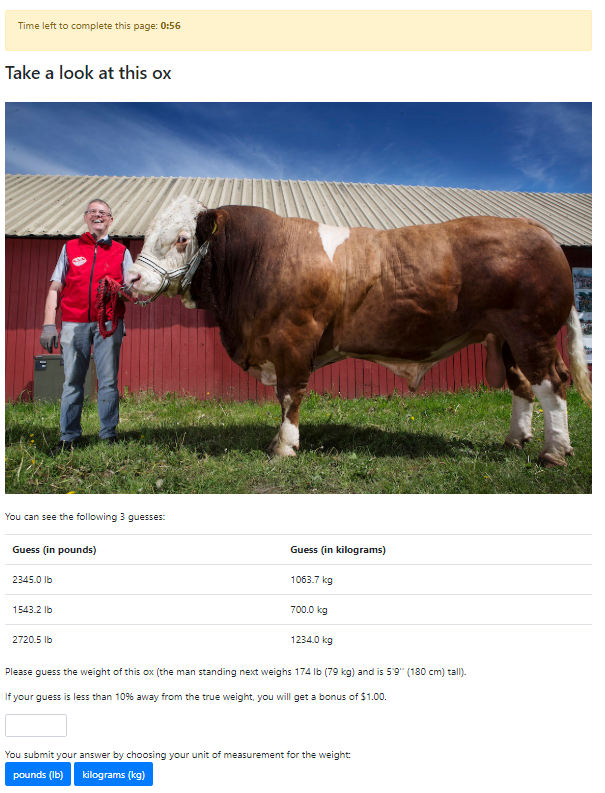
\includegraphics[width=.8\textwidth]{../Screenshots/FigS1.png}
\caption{Screendump of the choice-page in the dot-experiment with $d=403$ and $v=9$.}
\label{fig:S1}
\end{figure}


\begin{figure}%[!h]
	\begin{subfigure}[b]{.8\textwidth}
		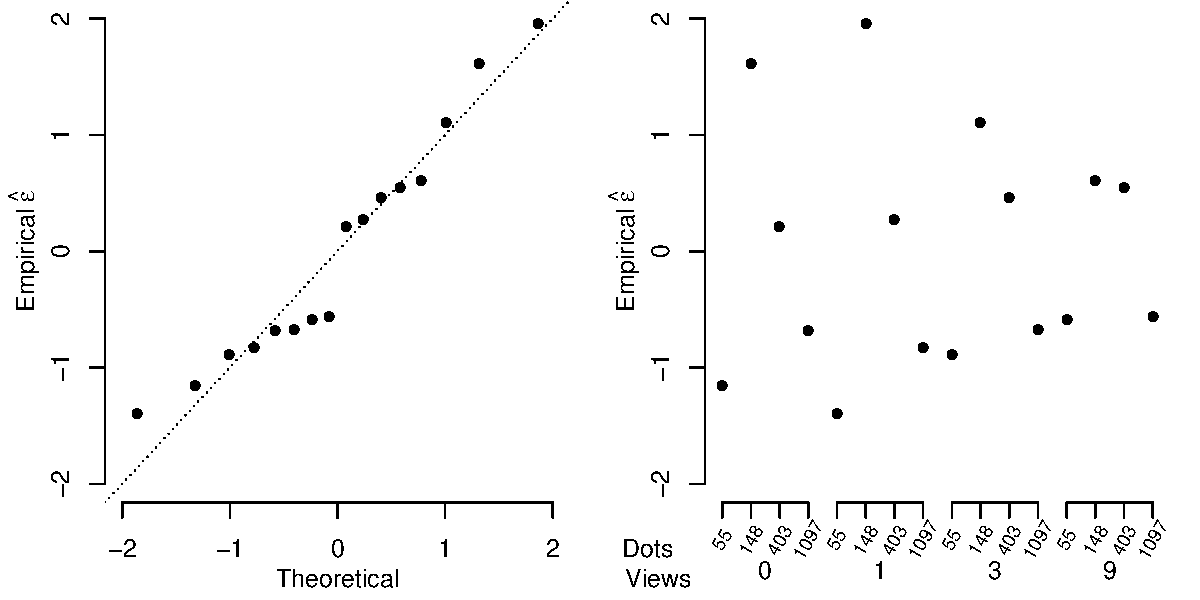
\includegraphics[width=\textwidth]{med_residual_h.pdf}
	\end{subfigure}
	\begin{subfigure}[b]{.8\textwidth}
		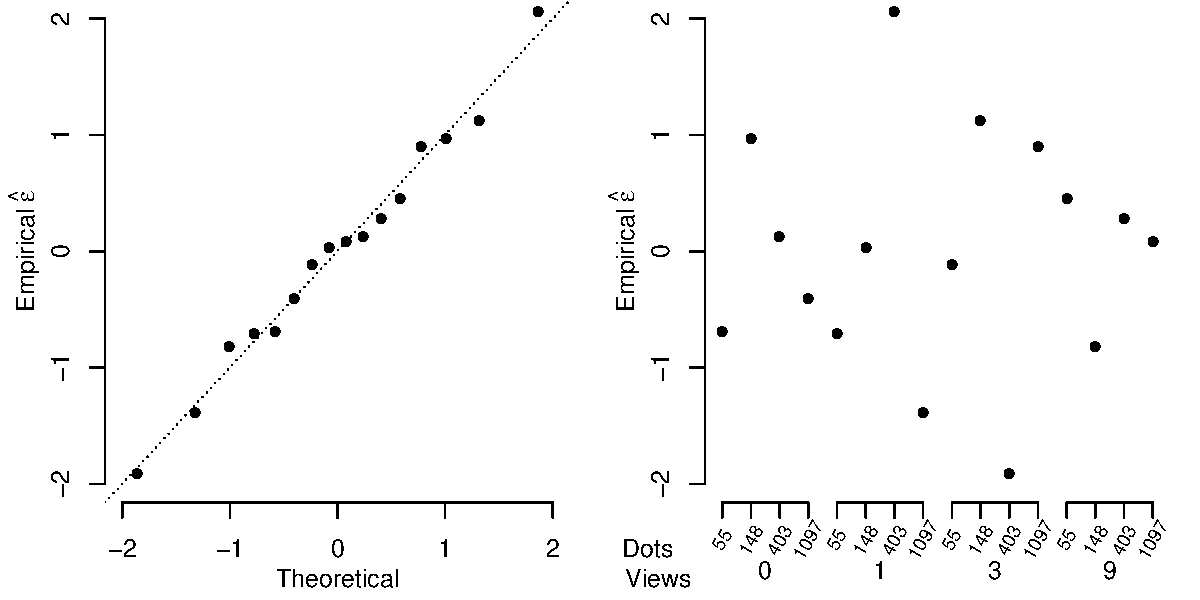
\includegraphics[width=\textwidth]{med_residual_m.pdf}	
	\end{subfigure}
	\caption{Model diagnostic plots for median analysis. Top left: QQ plot for the residuals from the historical thread medians analysis. Top right: the same residuals plottet against session groups. Bottom left: QQ plot for the residuals from the manipulated thread medians analysis. Bottom right: the same residuals plottet against session groups.}
	\label{fig: qq plots median}
\end{figure}


\begin{figure}%[!h]
\centering
	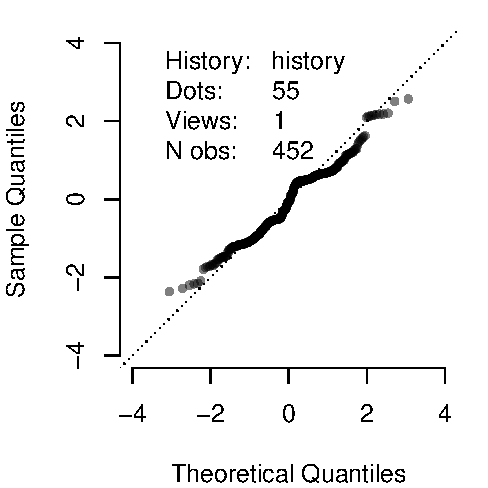
\includegraphics[width=.195\linewidth]{qqplots/qqplot_1}
	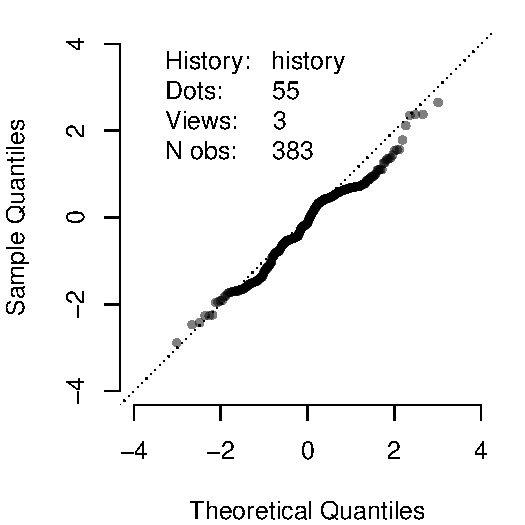
\includegraphics[width=.195\linewidth]{qqplots/qqplot_2}
	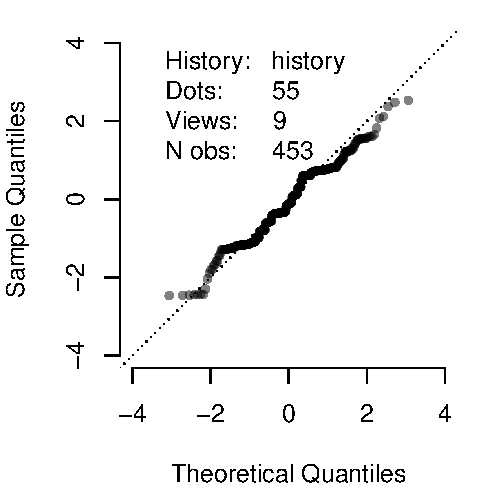
\includegraphics[width=.195\linewidth]{qqplots/qqplot_3}
	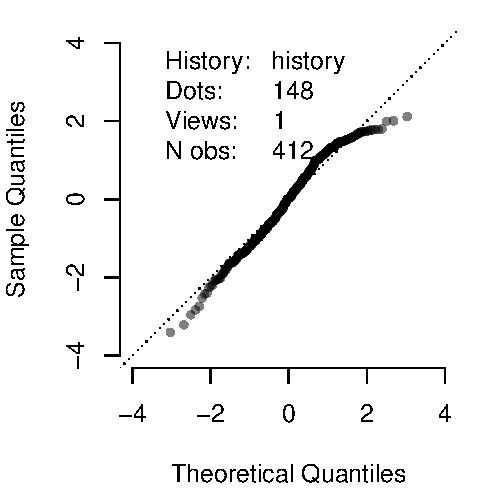
\includegraphics[width=.195\linewidth]{qqplots/qqplot_4}		
	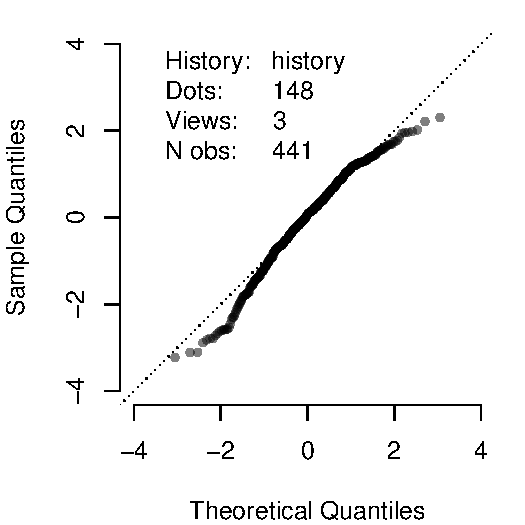
\includegraphics[width=.195\linewidth]{qqplots/qqplot_5}
	
	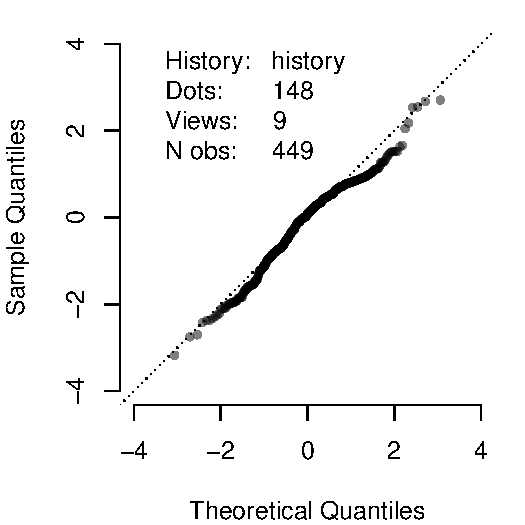
\includegraphics[width=.195\linewidth]{qqplots/qqplot_6}
	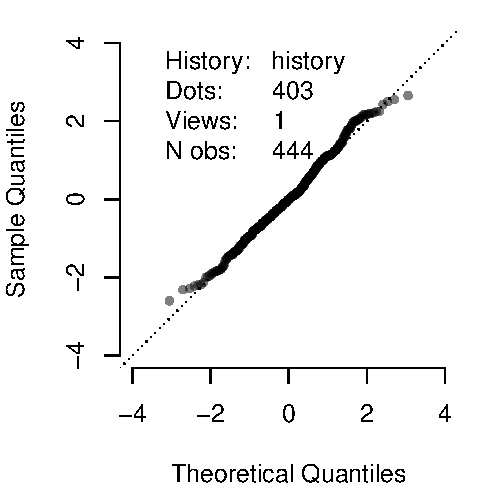
\includegraphics[width=.195\linewidth]{qqplots/qqplot_7}
	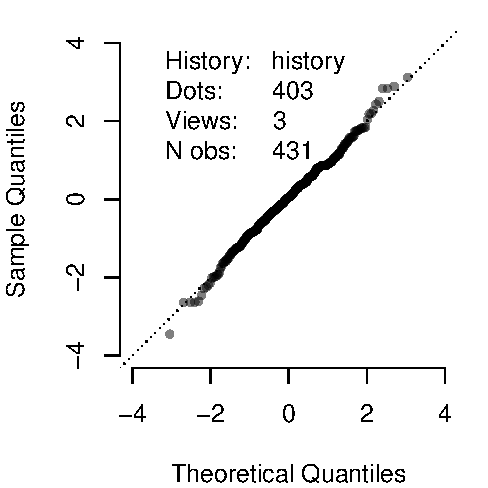
\includegraphics[width=.195\linewidth]{qqplots/qqplot_8}
	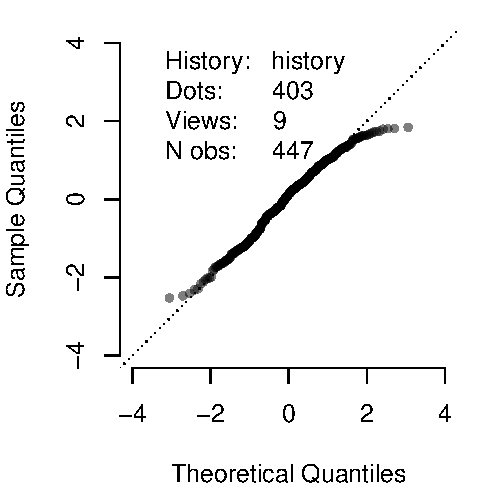
\includegraphics[width=.195\linewidth]{qqplots/qqplot_9}		
	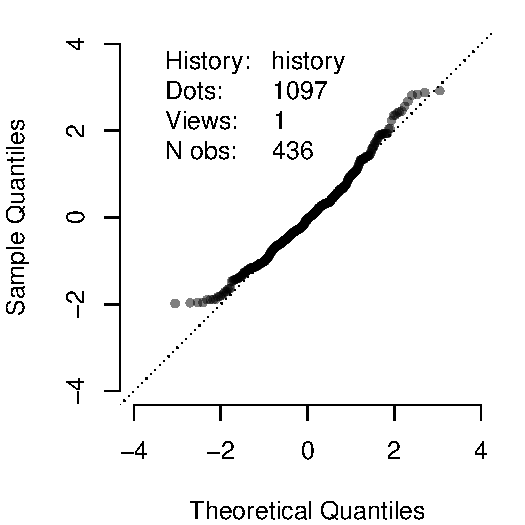
\includegraphics[width=.195\linewidth]{qqplots/qqplot_10}		

	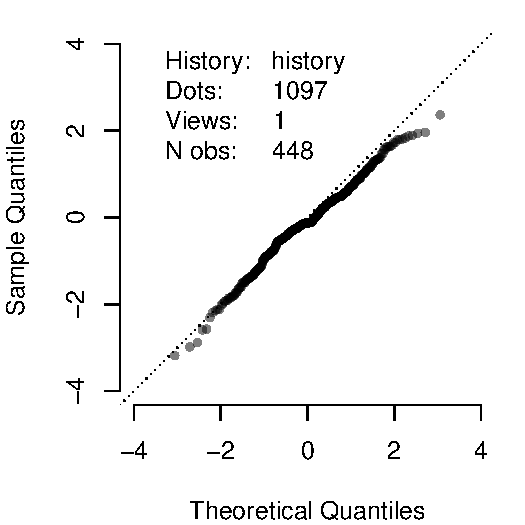
\includegraphics[width=.195\linewidth]{qqplots/qqplot_11}
	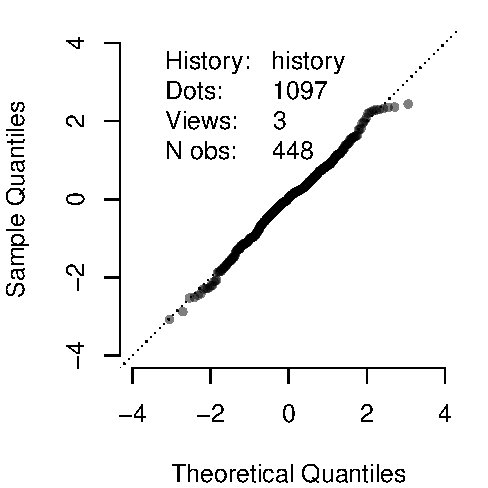
\includegraphics[width=.195\linewidth]{qqplots/qqplot_12}
	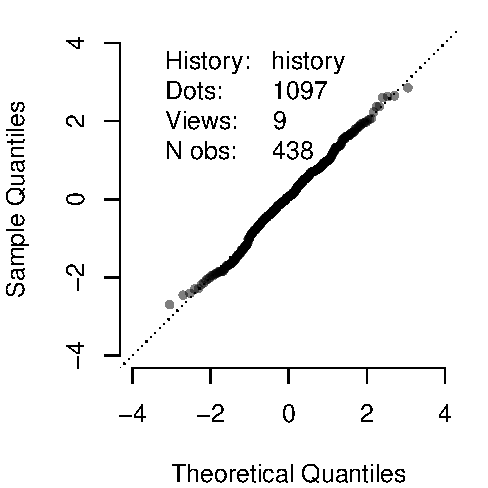
\includegraphics[width=.195\linewidth]{qqplots/qqplot_13}
	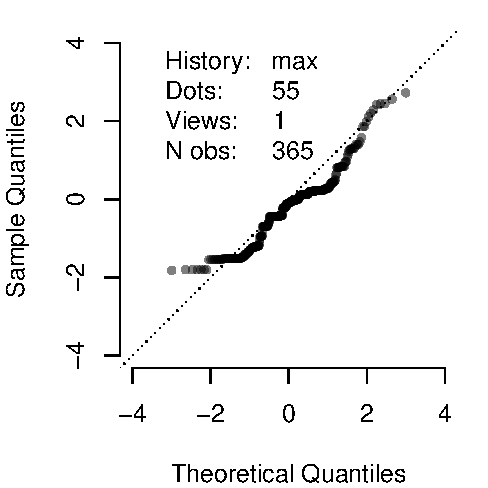
\includegraphics[width=.195\linewidth]{qqplots/qqplot_14}		
	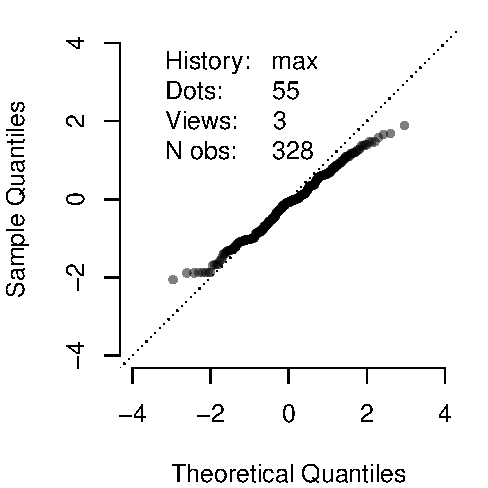
\includegraphics[width=.195\linewidth]{qqplots/qqplot_15}
	
	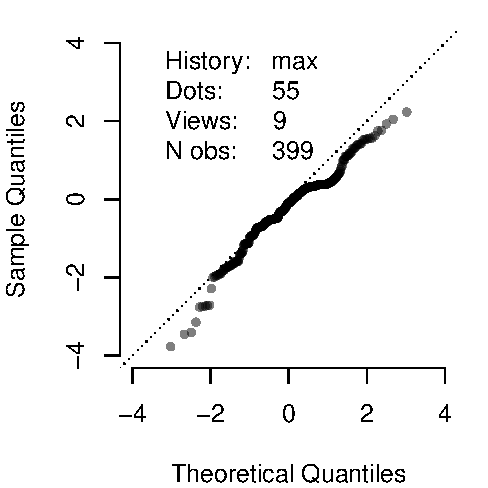
\includegraphics[width=.195\linewidth]{qqplots/qqplot_16}
	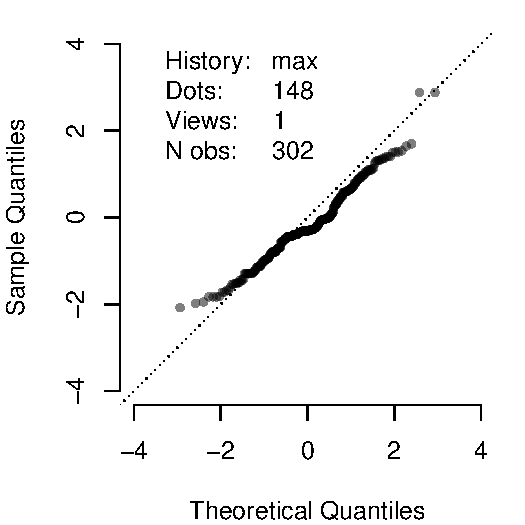
\includegraphics[width=.195\linewidth]{qqplots/qqplot_17}
	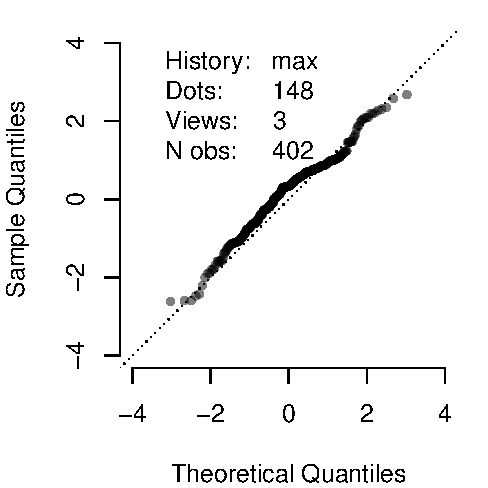
\includegraphics[width=.195\linewidth]{qqplots/qqplot_18}
	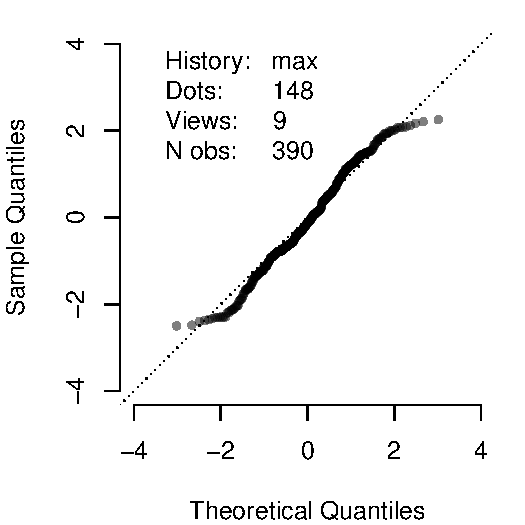
\includegraphics[width=.195\linewidth]{qqplots/qqplot_19}		
	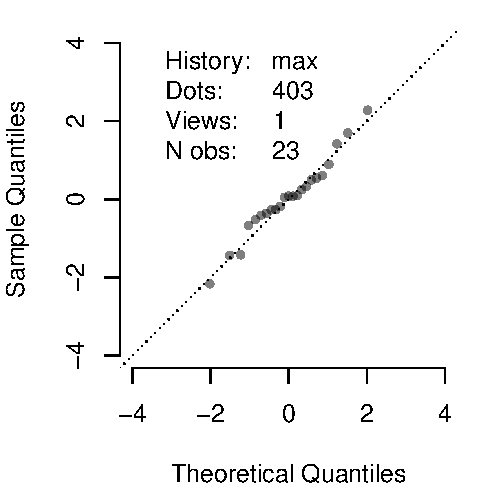
\includegraphics[width=.195\linewidth]{qqplots/qqplot_20}
	
	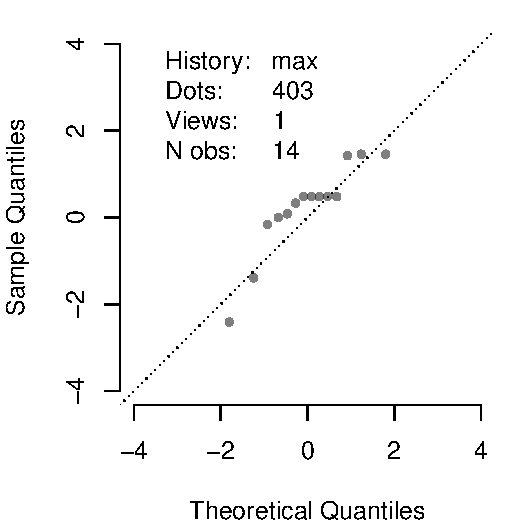
\includegraphics[width=.195\linewidth]{qqplots/qqplot_21}
	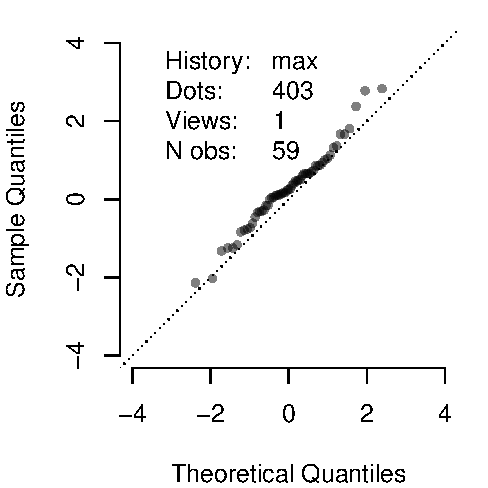
\includegraphics[width=.195\linewidth]{qqplots/qqplot_22}
	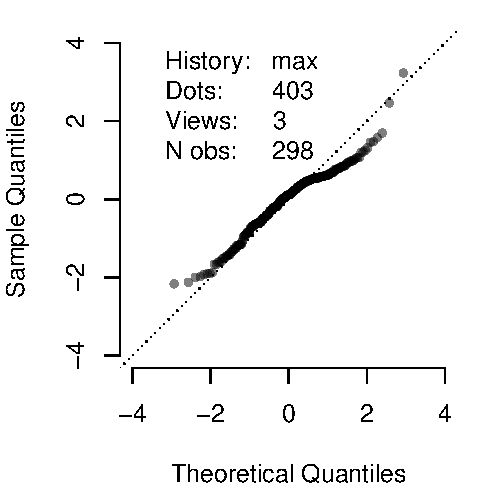
\includegraphics[width=.195\linewidth]{qqplots/qqplot_23}
	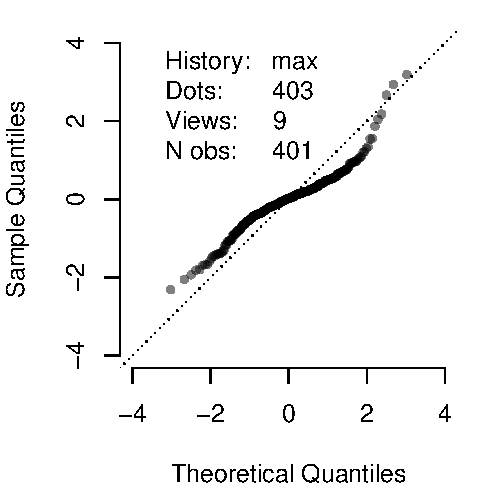
\includegraphics[width=.195\linewidth]{qqplots/qqplot_24}		
	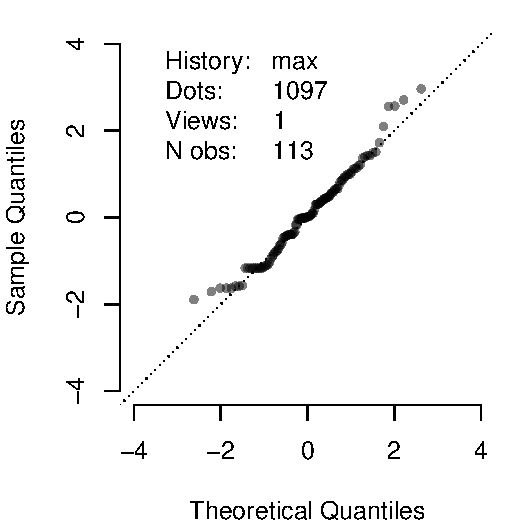
\includegraphics[width=.195\linewidth]{qqplots/qqplot_25}
	
	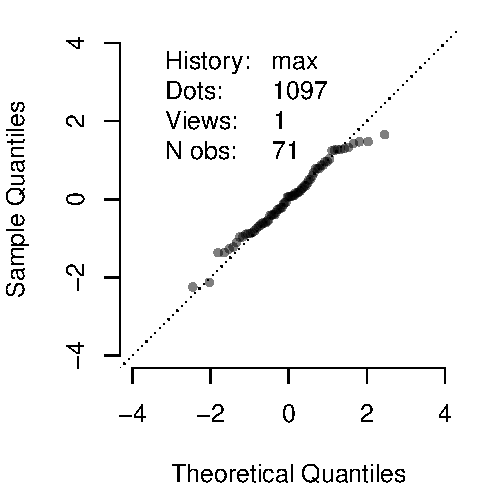
\includegraphics[width=.195\linewidth]{qqplots/qqplot_26}
	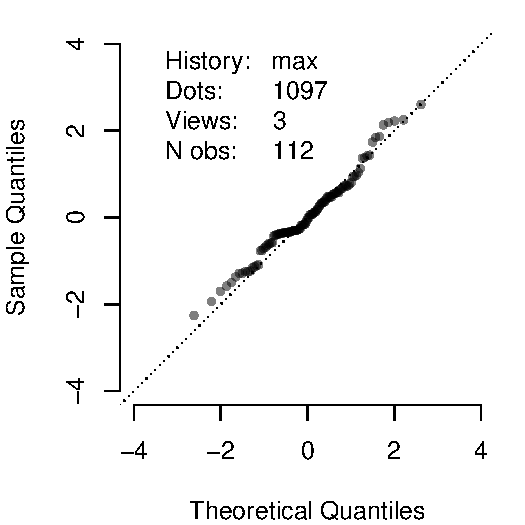
\includegraphics[width=.195\linewidth]{qqplots/qqplot_27}
	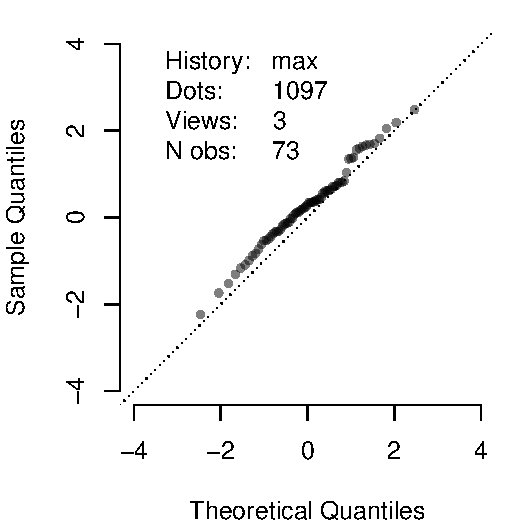
\includegraphics[width=.195\linewidth]{qqplots/qqplot_28}
	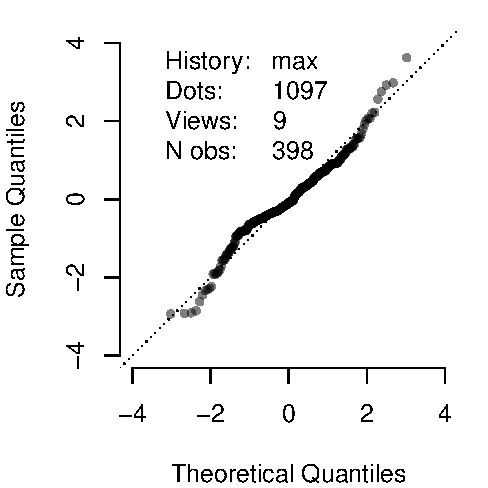
\includegraphics[width=.195\linewidth]{qqplots/qqplot_29}	
	\caption{QQ-plots for the 29 unique threads from Amazon Mechanical Turk experiments. With some exceptions, the models fit fairly well. Some series with very few observations are discarded in the analysis.}\label{fig: QQ plots AMT}
\end{figure}

\begin{figure}[!h]
\centering
	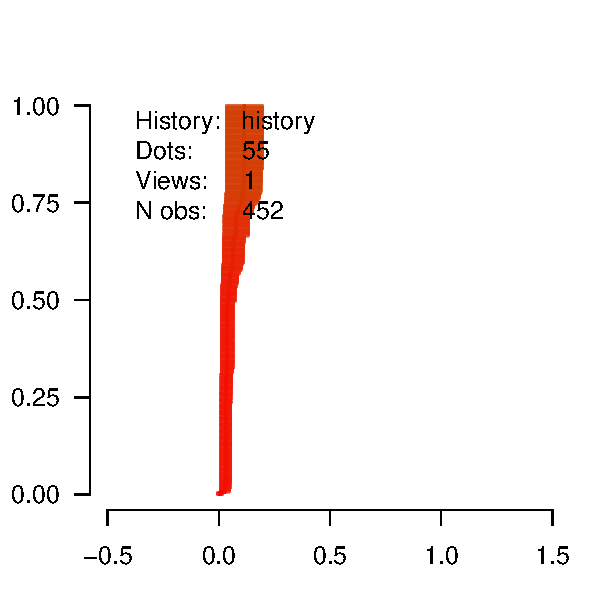
\includegraphics[width=.195\linewidth]{betas/beta_plot_1}
	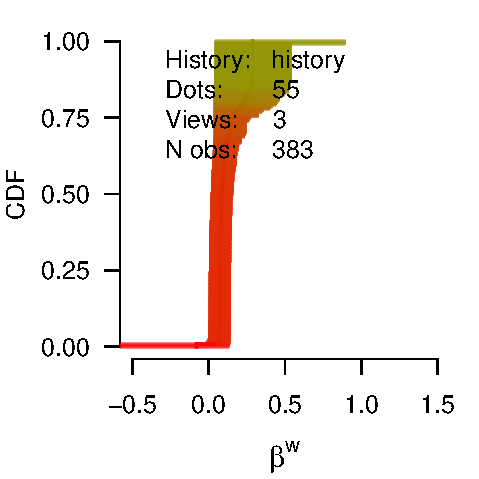
\includegraphics[width=.195\linewidth]{betas/beta_plot_2}
	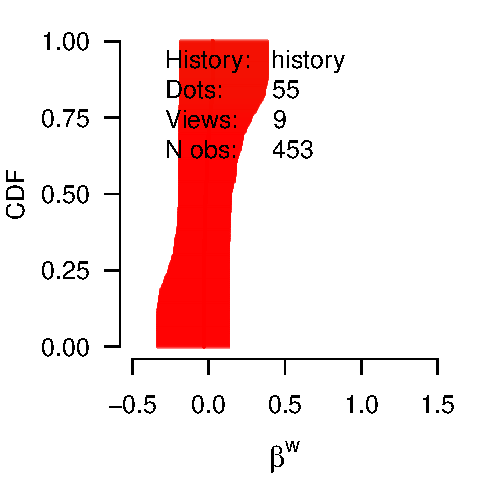
\includegraphics[width=.195\linewidth]{betas/beta_plot_3}
	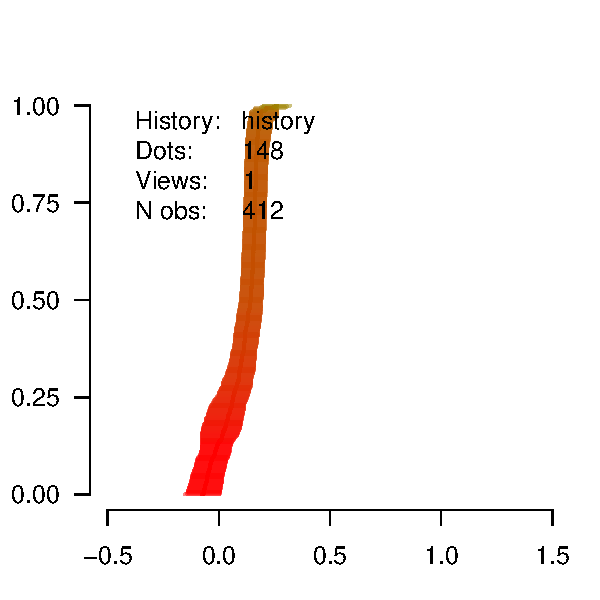
\includegraphics[width=.195\linewidth]{betas/beta_plot_4}		
	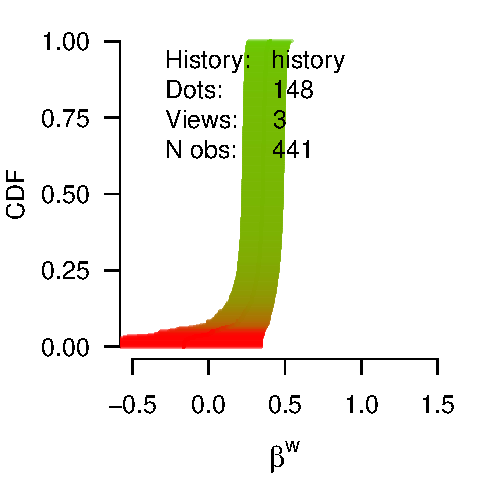
\includegraphics[width=.195\linewidth]{betas/beta_plot_5}
	
	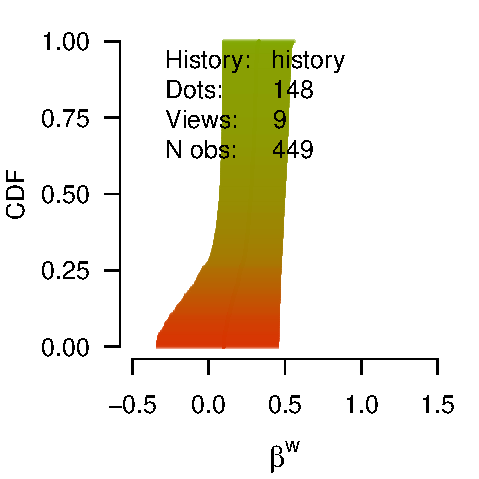
\includegraphics[width=.195\linewidth]{betas/beta_plot_6}
	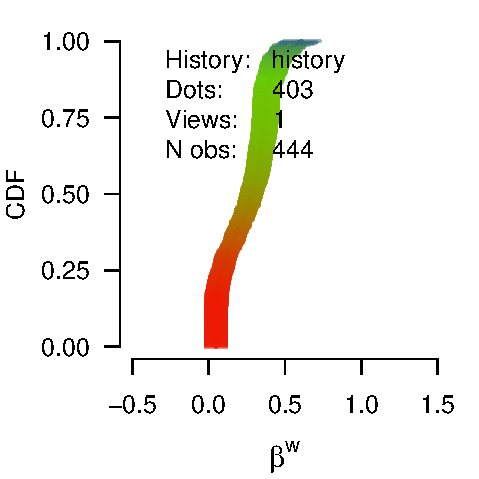
\includegraphics[width=.195\linewidth]{betas/beta_plot_7}
	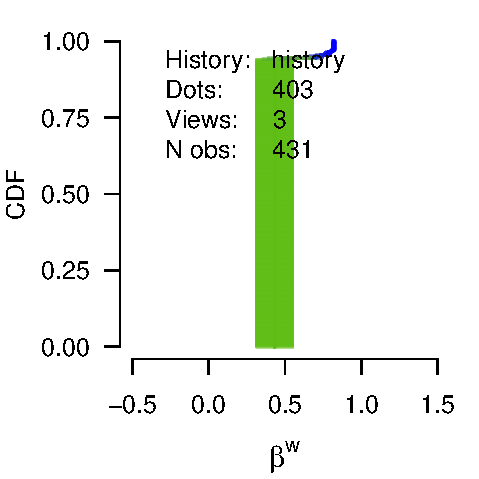
\includegraphics[width=.195\linewidth]{betas/beta_plot_8}
	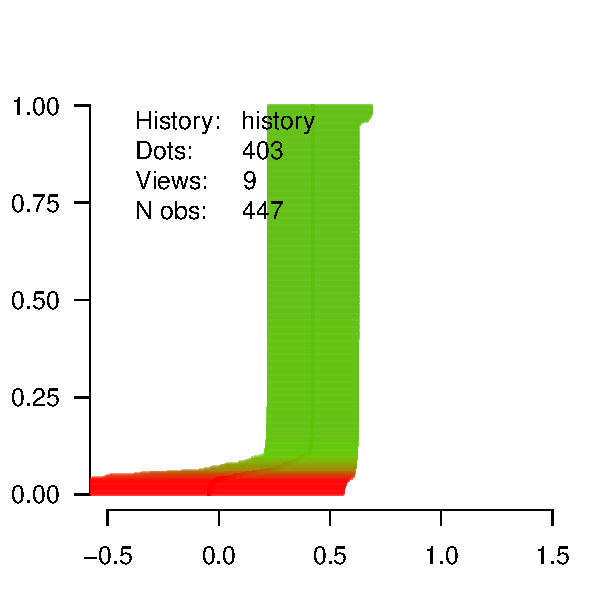
\includegraphics[width=.195\linewidth]{betas/beta_plot_9}		
	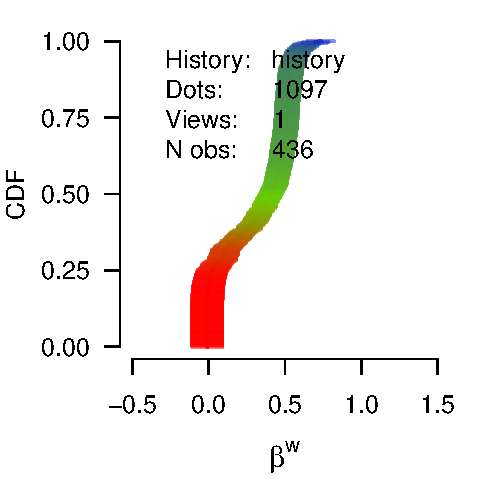
\includegraphics[width=.195\linewidth]{betas/beta_plot_10}		

	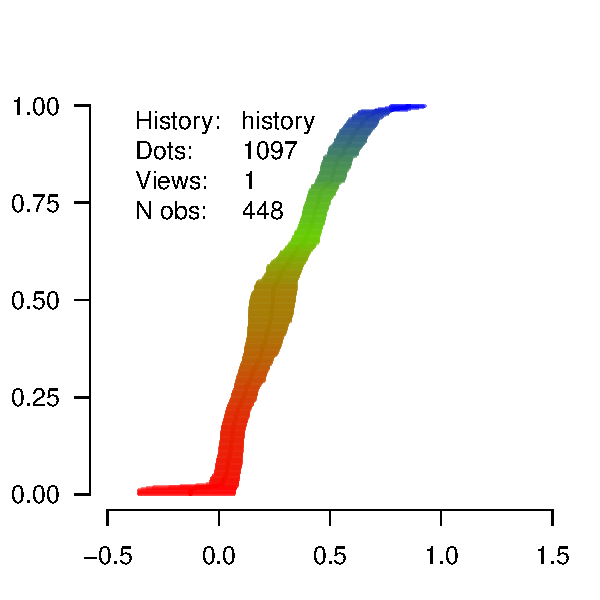
\includegraphics[width=.195\linewidth]{betas/beta_plot_11}
	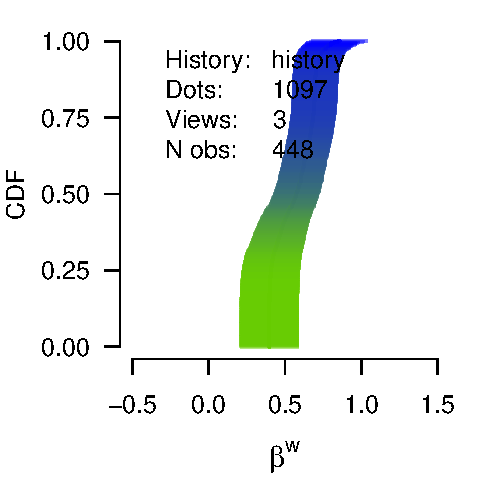
\includegraphics[width=.195\linewidth]{betas/beta_plot_12}
	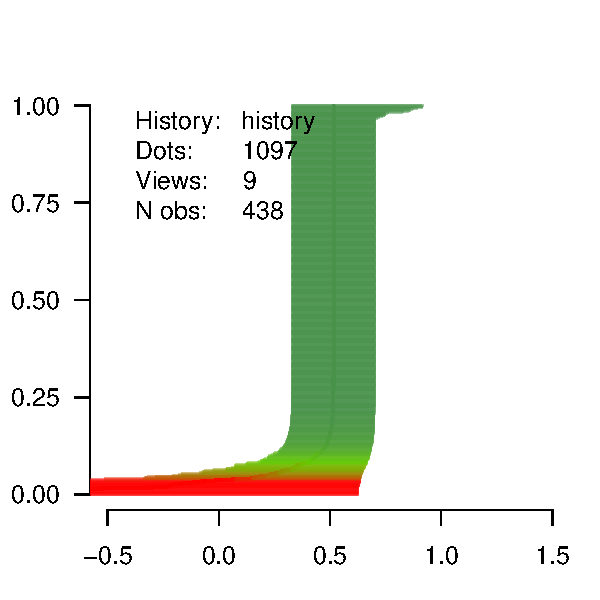
\includegraphics[width=.195\linewidth]{betas/beta_plot_13}
	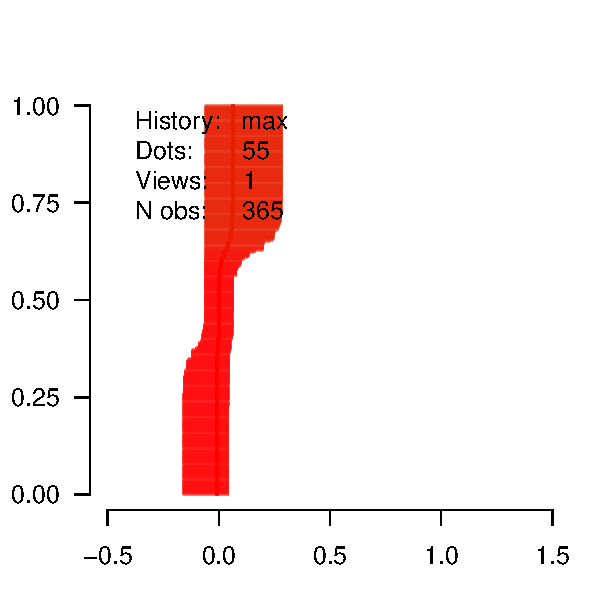
\includegraphics[width=.195\linewidth]{betas/beta_plot_14}		
	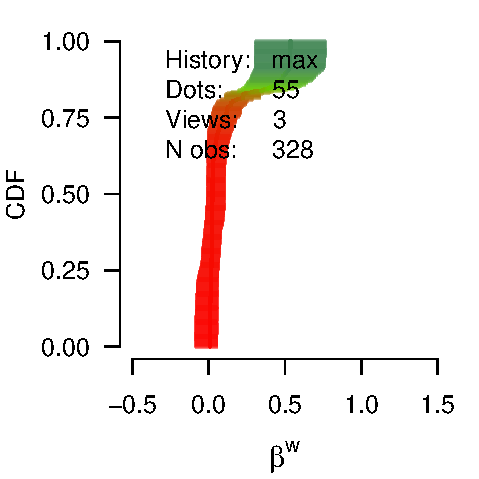
\includegraphics[width=.195\linewidth]{betas/beta_plot_15}
	
	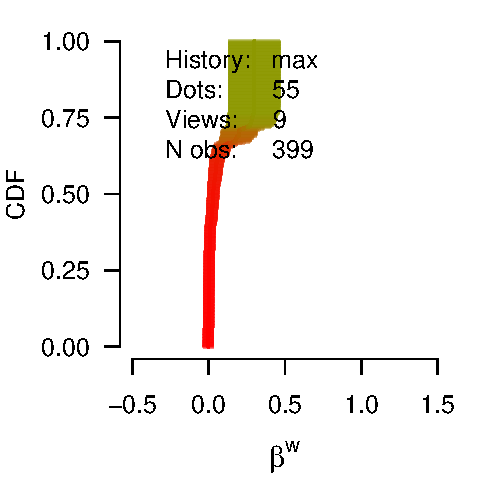
\includegraphics[width=.195\linewidth]{betas/beta_plot_16}
	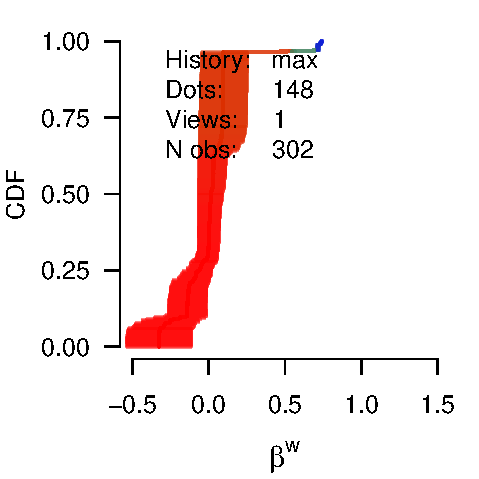
\includegraphics[width=.195\linewidth]{betas/beta_plot_17}
	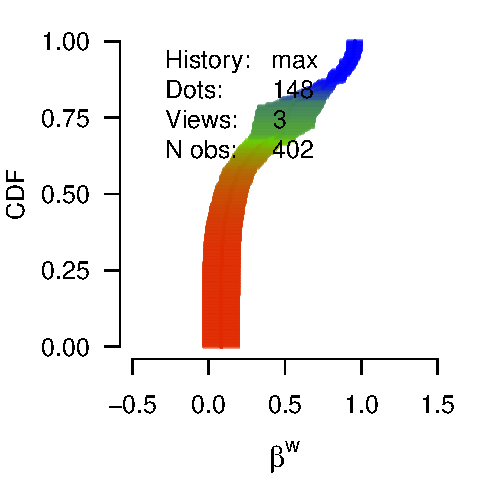
\includegraphics[width=.195\linewidth]{betas/beta_plot_18}
	\includegraphics[width=.195\linewidth]{betas/beta_plot_19}		
	\includegraphics[width=.195\linewidth]{betas/beta_plot_20}
	
	\includegraphics[width=.195\linewidth]{betas/beta_plot_21}
	\includegraphics[width=.195\linewidth]{betas/beta_plot_22}
	\includegraphics[width=.195\linewidth]{betas/beta_plot_23}
	\includegraphics[width=.195\linewidth]{betas/beta_plot_24}		
	\includegraphics[width=.195\linewidth]{betas/beta_plot_25}
	
	\includegraphics[width=.195\linewidth]{betas/beta_plot_26}
	\includegraphics[width=.195\linewidth]{betas/beta_plot_27}
	\includegraphics[width=.195\linewidth]{betas/beta_plot_28}
	\includegraphics[width=.195\linewidth]{betas/beta_plot_29}	
	\caption{$\beta^w$'s.}\label{fig: weighted beta distributions}
\end{figure}

\begin{figure}[!h]
\centering
	\includegraphics[width=.195\linewidth]{threads/thread_plot_1}
	\includegraphics[width=.195\linewidth]{threads/thread_plot_2}
	\includegraphics[width=.195\linewidth]{threads/thread_plot_3}
	\includegraphics[width=.195\linewidth]{threads/thread_plot_4}		
	\includegraphics[width=.195\linewidth]{threads/thread_plot_5}
	
	\includegraphics[width=.195\linewidth]{threads/thread_plot_6}
	\includegraphics[width=.195\linewidth]{threads/thread_plot_7}
	\includegraphics[width=.195\linewidth]{threads/thread_plot_8}
	\includegraphics[width=.195\linewidth]{threads/thread_plot_9}		
	\includegraphics[width=.195\linewidth]{threads/thread_plot_10}		

	\includegraphics[width=.195\linewidth]{threads/thread_plot_11}
	\includegraphics[width=.195\linewidth]{threads/thread_plot_12}
	\includegraphics[width=.195\linewidth]{threads/thread_plot_13}
	\includegraphics[width=.195\linewidth]{threads/thread_plot_14}		
	\includegraphics[width=.195\linewidth]{threads/thread_plot_15}
	
	\includegraphics[width=.195\linewidth]{threads/thread_plot_16}
	\includegraphics[width=.195\linewidth]{threads/thread_plot_17}
	\includegraphics[width=.195\linewidth]{threads/thread_plot_18}
	\includegraphics[width=.195\linewidth]{threads/thread_plot_19}		
	\includegraphics[width=.195\linewidth]{threads/thread_plot_20}
	
	%\includegraphics[width=.195\linewidth]{threads/thread_plot_21}
	\includegraphics[width=.195\linewidth]{betas/beta_plot_21}
	\includegraphics[width=.195\linewidth]{threads/thread_plot_22}
	\includegraphics[width=.195\linewidth]{threads/thread_plot_23}
	\includegraphics[width=.195\linewidth]{threads/thread_plot_24}		
	\includegraphics[width=.195\linewidth]{threads/thread_plot_25}
	
	\includegraphics[width=.195\linewidth]{threads/thread_plot_26}
	\includegraphics[width=.195\linewidth]{threads/thread_plot_27}
	\includegraphics[width=.195\linewidth]{threads/thread_plot_28}
	\includegraphics[width=.195\linewidth]{threads/thread_plot_29}	
	\caption{Threads}\label{fig: threads with social info and colored by beta weights}
\end{figure}

\begin{figure}[!h]
\centering
	\includegraphics[width=.195\linewidth]{info/info_plot_1}
	\includegraphics[width=.195\linewidth]{info/info_plot_2}
	\includegraphics[width=.195\linewidth]{info/info_plot_3}
	\includegraphics[width=.195\linewidth]{info/info_plot_4}		
	\includegraphics[width=.195\linewidth]{info/info_plot_5}
	
	\includegraphics[width=.195\linewidth]{info/info_plot_6}
	\includegraphics[width=.195\linewidth]{info/info_plot_7}
	\includegraphics[width=.195\linewidth]{info/info_plot_8}
	\includegraphics[width=.195\linewidth]{info/info_plot_9}		
	\includegraphics[width=.195\linewidth]{info/info_plot_10}		

	\includegraphics[width=.195\linewidth]{info/info_plot_11}
	\includegraphics[width=.195\linewidth]{info/info_plot_12}
	\includegraphics[width=.195\linewidth]{info/info_plot_13}
	\includegraphics[width=.195\linewidth]{info/info_plot_14}		
	\includegraphics[width=.195\linewidth]{info/info_plot_15}
	
	\includegraphics[width=.195\linewidth]{info/info_plot_16}
	\includegraphics[width=.195\linewidth]{info/info_plot_17}
	\includegraphics[width=.195\linewidth]{info/info_plot_18}
	\includegraphics[width=.195\linewidth]{info/info_plot_19}		
	\includegraphics[width=.195\linewidth]{info/info_plot_20}
	
	%\includegraphics[width=.195\linewidth]{info/info_plot_21}
	\includegraphics[width=.195\linewidth]{betas/beta_plot_21}
	\includegraphics[width=.195\linewidth]{info/info_plot_22}
	\includegraphics[width=.195\linewidth]{info/info_plot_23}
	\includegraphics[width=.195\linewidth]{info/info_plot_24}		
	\includegraphics[width=.195\linewidth]{info/info_plot_25}
	
	\includegraphics[width=.195\linewidth]{info/info_plot_26}
	\includegraphics[width=.195\linewidth]{info/info_plot_27}
	\includegraphics[width=.195\linewidth]{info/info_plot_28}
	\includegraphics[width=.195\linewidth]{info/info_plot_29}	
	\caption{Info.}\label{fig: social info vs estimates}
\end{figure}

\begin{figure}[!h]
\centering
	\includegraphics[width=.5\linewidth]{betascale_horizontal}
	\caption{Color scale for $\beta^w$.}\label{fig: beta scale}
\end{figure}

\begin{figure}
\centering
\includegraphics[width=1\linewidth]{summary_stats_plot.pdf}
\caption{\textbf{Left:} Summary statistics of $d \times v$ history treatments with a total of 7.814 magnitude estimates of the number of dots in an image, $d \in \{55,148,403,1097\}$, while participants are able to see $v \in \{0,1,3,9\}$ preceding estimates. Greys are the control treatments with $v=0$. Estimates are log-transformed. Large circles indicate medians, triangles indicate arithmetic means, thick lines show interquartile ranges, thin lines show interdecile ranges, vertical black lines show the true value, and stars indicate significance levels compared to the control treatment (two-sided Wilcoxon-Mann-Whitney test). No outliers were removed, making the arithmetic means strongly right skewed. \textbf{Right:} Summary statistics of $d \times v$ treatments with a total of 3.934 additional magnitude estimates, where participants do not see the preceding estimates but the $v \in \{1,3,9\}$ \textit{highest} estimates made so far. The controls, $v=0$, are the same as on the left hand side.}\label{fig:sum_stats}
\end{figure}


\begin{figure}
	\centering
	\begin{subfigure}{.44\linewidth}
		\includegraphics[width=.7\linewidth]{thread_history_1097_1.pdf}	
		\includegraphics[width=.28\linewidth]{beta_history_1097_1.pdf}	
		\includegraphics[width=.7\linewidth]{thread_history_1097_1_extra.pdf}	
		\includegraphics[width=.28\linewidth]{beta_history_1097_1_extra.pdf}
		\includegraphics[width=.7\linewidth]{thread_history_1097_1_extra.pdf}	
		\includegraphics[width=.28\linewidth]{beta_history_1097_1_extra.pdf}
		\includegraphics[width=.7\linewidth]{thread_history_1097_1_extra.pdf}	
		\includegraphics[width=.28\linewidth]{beta_history_1097_1_extra.pdf}
		\caption{\footnotesize History thread with with increasing $d$ and $v$}
		\label{fig:supp hist}
	\end{subfigure}
	\begin{subfigure}{.44\linewidth}
		\includegraphics[width=.7\linewidth]{thread_max_55_1.pdf}
		\includegraphics[width=.28\linewidth]{beta_max_55_1.pdf}	
		\includegraphics[width=.7\linewidth]{thread_max_55_3.pdf}
		\includegraphics[width=.28\linewidth]{beta_max_55_3.pdf}
		\includegraphics[width=.7\linewidth]{thread_max_55_3.pdf}
		\includegraphics[width=.28\linewidth]{beta_max_55_3.pdf}
		%\includegraphics[width=.7\linewidth]{thread_max_148_3.pdf}
		%\includegraphics[width=.8\linewidth]{threads/thread_plot_24}
		\includegraphics[width=.7\linewidth]{thread_max_1097_9.pdf}
		\includegraphics[width=.28\linewidth]{beta_max_1097_9.pdf}
		\caption{\footnotesize Manipulated thread with with increasing $d$ and $v$}
		\label{fig:supp max}
	\end{subfigure}
	\caption{new caption}
\label{fig:more}
\end{figure}



\begin{figure}
	\centering
	\begin{subfigure}{1\linewidth}
		\centering
		\includegraphics[width=1\linewidth]{beta_history}
		\caption{\footnotesize History}
		\label{fig: betaw history}
	\end{subfigure}
	\begin{subfigure}{1\linewidth}
		\centering
		\includegraphics[width=1\linewidth]{beta_max}
		\caption{\footnotesize Manipulated}
		\label{fig: betaw manipulated}
	\end{subfigure}
	\caption{Comparison of persuadability scores, $\beta^w$, for individuals participating in more than one study. For each participant on the x-axis there are 2-4 dots of the same color, which is determined by the average $\beta^w$ score, also shown by the solid line.}
	\label{fig: betaw comparisons}
\end{figure}

\newpage

\begin{table}\centering
\caption{Data Table of all threads. Legend: $d \in \{55, 148, 403, 1097\}$; $v$ = view count; method: \'history\'-threads show the preceding estimates as they have been recorded in the thread; N = thread length; median = median of thread; mean = mean of thread; SD = standard deviation; CV = coefficient of variation; skew = skewness; kurt = kurtosis; bonus = percentage of estimates within 10 \% of the true value, $d$.}

\begin{tabular}{lrrlrrrrrrrr}
\hline
 method   &    d &   v & thread   &   N &   median &     mean &       SD &    CV &   skew &   kurt &   bonus (\%) \\
\hline
 history  &   55 &   0 & fscmakcz & 464 &     55   &  2360.57 & 42038.6  & 17.81 &  21.01 & 445.08 &        60.99 \\
 history  &   55 &   1 & hs6bovtz & 477 &     57   &  1682.13 & 29381.7  & 17.47 &  21.18 & 453.74 &        57.02 \\
 history  &   55 &   3 & 3cda8qpn & 405 &     56   &  8320.59 & 73524.4  &  8.84 &   9.59 &  93.58 &        66.91 \\
 history  &   55 &   9 & bvpj37io & 476 &     56   &  1239.85 & 25435.5  & 20.51 &  21.74 & 470.87 &        56.09 \\
 history  &  148 &   0 & dwnjf9mb & 464 &    140   &  1349.14 & 12891    &  9.55 &  12.83 & 172.18 &        22.41 \\
 history  &  148 &   1 & ehaxc7lu & 435 &    150   &  2250.86 & 27802.5  & 12.35 &  15.66 & 261.32 &        25.75 \\
 history  &  148 &   3 & ck291lk5 & 466 &    147.5 &  2523.51 & 38071.3  & 15.09 &  20.42 & 427.38 &        23.18 \\
 history  &  148 &   9 & 2hxe3g0w & 473 &    153   &  3182.51 & 38085.7  & 11.97 &  13.85 & 196.79 &        24.52 \\
 history  &  403 &   0 & hqx0v7t5 & 473 &    300   &  4816.02 & 49624.9  & 10.3  &  14.16 & 220.03 &         7.82 \\
 history  &  403 &   1 & 9bbkjlye & 469 &    320   &  2791.59 & 31667.6  & 11.34 &  15.23 & 248.43 &         8.1  \\
 history  &  403 &   3 & 5du4txa7 & 455 &    350   &  2430    & 29944.3  & 12.32 &  15.25 & 233.19 &        11.65 \\
 history  &  403 &   9 & spw8qdcd & 470 &    400   &  3035.65 & 36078.8  & 11.89 &  15.32 & 235.27 &        10.43 \\
 history  & 1097 &   0 & hal5jdl0 & 423 &    657   &  8855.13 & 76379.1  &  8.63 &  11.46 & 138.21 &         9.69 \\
 history  & 1097 &   1 & huyygtho & 461 &    750   &  2924.95 & 25012.2  &  8.55 &  17.91 & 344.84 &         9.76 \\
 history  & 1097 &   1 & z0rvh02v & 473 &    650   &  8091.24 & 68728.9  &  8.49 &  11.74 & 144.62 &         8.67 \\
 history  & 1097 &   3 & hhb0if6e & 470 &    812.5 &  4811.97 & 53329.9  & 11.08 &  15.61 & 259.91 &        20.64 \\
 history  & 1097 &   9 & wv4xujg7 & 460 &    999   &  2748    & 31206.8  & 11.36 &  21.24 & 451.09 &        13.7  \\
 max      &   55 &   1 & aebicytb & 384 &     57   &    68.7  &    35.77 &  0.52 &   2.82 &   8.76 &        54.17 \\
 max      &   55 &   3 & 094p61xp & 340 &     60   &   101.05 &   413.25 &  4.09 &  18    & 326.23 &        43.82 \\
 max      &   55 &   9 & 8c80yyxl & 418 &     60   &    75.03 &    45.69 &  0.61 &   4.72 &  34.23 &        51.44 \\
 max      &  148 &   1 & 78wuly7l & 317 &    152   &   271.06 &   323.75 &  1.19 &   3.84 &  19.06 &        17.03 \\
 max      &  148 &   3 & u2sxnl2p & 418 &    220   &   366.6  &   596    &  1.63 &  11.6  & 179.79 &         9.57 \\
 max      &  148 &   9 & mf57hnwb & 412 &    210   &   266.74 &   168.39 &  0.63 &   1.08 &   0.2  &        12.38 \\
 max      &  403 &   1 & 1r17post &  25 &    400   &   549    &   402.64 &  0.73 &   1.83 &   4.14 &         4    \\
 max      &  403 &   1 & 6c4s02ki &  16 &     90   &   452.5  &   614.18 &  1.36 &   2.26 &   4.85 &         0    \\
 max      &  403 &   1 & e8vv9575 &  64 &    600   &   734.38 &   506.71 &  0.69 &   0.48 &  -1    &         6.25 \\
 max      &  403 &   3 & ua2230ux & 315 &    600   &  3215.08 &  9635.18 &  3    &   4.84 &  22.79 &         8.25 \\
 max      &  403 &   9 & 1xyev3dj & 422 &    887.5 &  4758.88 & 25397.5  &  5.34 &  17.68 & 339.78 &         8.29 \\
 max      & 1097 &   1 & 7yqp8bxc & 116 &    800   &  5463.93 & 15517.2  &  2.84 &   4.21 &  16.95 &         8.62 \\
 max      & 1097 &   1 & q5brhgnz &  76 &   1062.5 &  3310.3  &  4690.72 &  1.42 &   2.13 &   4.19 &         5.26 \\
 max      & 1097 &   3 & 2x6km84z & 117 &   2500   &  7593.38 &  9341.25 &  1.23 &   1.29 &   0.35 &        13.68 \\
 max      & 1097 &   3 & ud5vo371 &  78 &   2950   &  5167.06 & 12588.5  &  2.44 &   7.43 &  58.71 &         3.85 \\
 max      & 1097 &   9 & lh7wb36v & 416 &   3410   & 13024.2  & 38664.1  &  2.97 &  11.9  & 183.47 &         8.17 \\
\hline
 &&&& 11.748 &&&&&&& \\
\bottomrule
\end{tabular}
\end{table}\label{table:S1}

%%% Add this line AFTER all your figures and tables
\FloatBarrier

\dataset{dots.csv}{Anonymized data set of all dots-experiments. Parameters: task = type of experiment; $d$ = number of dots in image; $v$ = number of visible preceding estimates; session = thread name; hashed\_turker = anonymized participant id; decision order = order in which participants enter the queue; hist = list of guesses seen by participant; guess = estimate by participant}

\bibliography{wamot}
\end{document}